\section{DNS Fundamentals}

The DNS is used to resolve host names, making it possible to search for a name instead of an IP-address. This ensures that you can make a search for e.g. \url{www.google.com} and not get an error, even if they have changed IP-address at some point.

\subsection{Demonstration of DNS fundamentals - Linux}

The \textit{hostname} command shows the hostname of the system - in this case, it would just be \textbf{ubuntu}.\\

The \textit{nm-tool}, which is demonstrated below, is an utility that provides information about NetworkManager, devices, and wireless networks.

By running the command in a Linux terminal, we get the following output:

\begin{figure}[ht!]
\centering
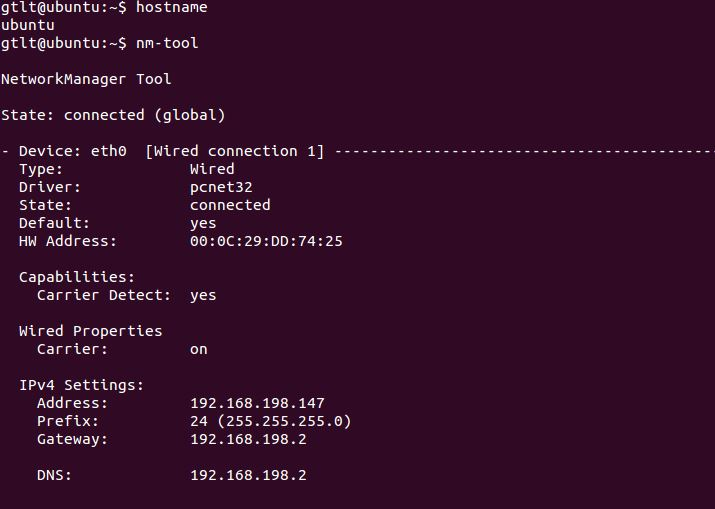
\includegraphics[width=150mm]{img/nm-tool.png}
\caption{Screenshot of running commands \textit{hostname} and \textit{nm-tool}}
\label{nm-tool}
\end{figure}

The \textit{Address} field tells us about the current internal IP-address for the device. The internal IP is an IP assigned for the device that is connected to a router. \\

The \textit{Prefix} tells us the number of significant bits used to identify a network. Subnet mask 255.255.255.0 has a prefix of 24 bits, which tells us that the first 24 bits identifies the network, and the last 8 bits identifies the specific machine. \\

The \textit{Gateway} field tells us about the IP-address for the current host router. In general, a gateway is a network point that acts as an entrance to another network. \\

The \textit{DNS} fields tells us which IP-address they connect to and make a lookup when accessing the internet.

\subsection{Demonstration of DNS fundamentals - in Windows}

It is also possible to view those fields in Windows, which can be done by opening a command window in Windows and then run the command \textit{ipconfig /all}. \\

This will demonstrate about pinging a webserver. Ping is a computer network administration utility used to test the reachability of a host on an Internet Protocol (IP) network and to measure the round-trip time for messages sent from the originating host to a destination computer.
We will experiment with \url{www.dr.dk} and then type in the IP-address in a webbrowser - it \underline{will} show the same result:

\begin{figure}[ht!]
\centering
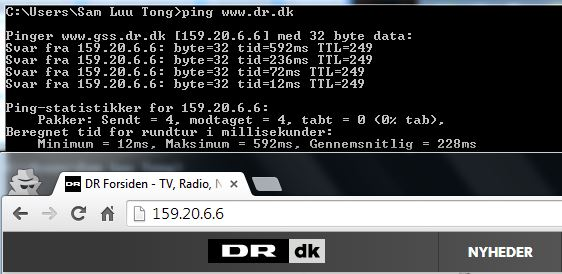
\includegraphics[width=150mm]{img/ping.png}
\caption{Screenshot of pinging www.dr.dk}
\label{ping}
\end{figure}

So whether we type \url{www.dr.dk} or we type 159.20.6.6 doesn't make a difference - only that \url{www.dr.dk} probably is easier to remember! \\

\subsection{Host Lookup Table - Background and demonstration}

\subsubsection{The Background}
Before DNS was fully deployed, a woman, \textbf{Peggy Karp}, created a lookup table that mapped all of the network resources in one text formatted file. This formatted file was a simple ASCII text file called “HOSTS.TXT”, and the table contained all of the hostnames and their related IP addresses.

Operators would install this file on their local server, which would then gain the capability to perform the requisite lookups locally and enable the computer to find resources out on the larger network without a lot of overhead. Whenever an operator added a new machine to the network, they would complete an email template with the appropriate information, send it off to the appropriate people at Stanford Research Institute (SRI) who would compile all of the changes and include them in the next release of HOSTS.TXT and store the new file on a globally available FTP server.

Operators would retrieve the updated versions on a regular basis and install them on their local servers. The first version of this table was distributed in \textit{1971-1972}. While this arrangement worked well for a number of years, but it suffered from one systemic problem – it wasn’t scalable as the network grew in popularity and new hosts were added. Therefore, the size of HOSTS.TXT grew in direct relationship. For each host added, HOSTS.TXT added a new record, and if the operators did not update their records on a regular basis, HOSTS.TXT would grow out of date which led all sorts of confusion. On the brighter side, it led the engineers of the time to come to the conclusion that a new structure would have to be put into place to replace HOSTS.TXT.

\subsubsection{Demonstration}
The Hosts.txt file still exists (in Linux under the folder /etc) and can be used to locally map hostnames to IP-addresses. To demonstrate this, the hostname "numsefisk" has been mapped to the IP-address of \url{www.dr.dk}, which is 159.20.6.6:

\begin{figure}[ht!]
\centering
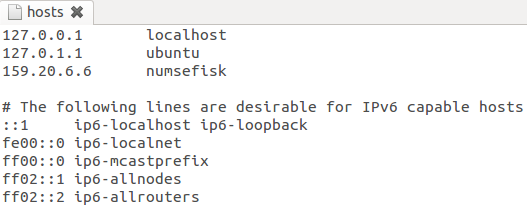
\includegraphics[width=150mm]{img/hostsText.png}
\caption{The change "numsefisk" made in Hosts.txt}
\label{hostsText}
\end{figure}

By running a browser and type "numsefisk", you will be redirected to www.dr.dk, or as an alternative, you could just ping "numsefisk" to test the changes.

It's worth knowing what happens first - is the HLT looked through before your primary DNS server is queried?
The answer can be found in host.conf, because this central file controls the resolver setup, which services to use and in what order. By opening the host.conf, the order is "host,bind", and therefore the HLT is looked through before the BIND DNS.

%Questions 4-7

\subsection{Top Level Domain}
To understand how DNS work, you have to consider some elements.\footnote{\url{https://archive.icann.org/en/tlds/}} If you look at an internet address, it is made of the www.second-level-domain.com, where the .com is the top level domain. The TLD defines in which TLD the router shall look for in the second-level-domain name.
The .com TLD is a generic TLD (gTLD), which states for which purpose they are to be used. It's worth to mention that Top Level Domains for different countries exist \footnote{These are called country codes Top Level Domain (ccTLD)} like .dk, .jp or .de.

\subsection{Fully Qualified Domain Name}
A domain name can be either fully qualified(FQDN) or not. The definition of a FQDN is its unambiguity, that is, it is unique, and there is only one interpretation of the domain. Hence also the dot at the end of a FQDN to define it is so e.g. \\ \url{http://www.dns-sd.org./TrailingDotsInDomainNames.html}.

\subsection{DNS zone and records}
A DNS zone is a portion of a Domain Name System, just like the area code in a post district. The zone has been delegated administrative responsibility for the DNS.

When a domain name is looked up,  a DNS zone returns a record, possibly a DNS "A" record. This depends on which record is needed to be returned considered the requested address. Records are data stored in the zone files of the DNS. An "A" record is a "Address record" that returns a 32-bit IPv4 address, most commonly used to map hostnames to an IP-address of the host.